\documentclass{article}
\usepackage[utf8]{inputenc}
\usepackage{xcolor}
\usepackage{hyperref}

\usepackage{rotating}

\usepackage{tabls}
\usepackage{booktabs}
\usepackage{amsmath}
\usepackage{amssymb}
\usepackage{amsthm}
\usepackage{amsfonts}
\usepackage{multicol}
\usepackage{enumitem}
\usepackage{microtype}
\usepackage{tikz}
\usepackage{pgfplots}
\usetikzlibrary{positioning}
\usepackage{multirow}

\usepackage{comment}

\usepackage{graphicx}
\usepackage{wrapfig}

\theoremstyle{plain}
\newtheorem{theorem}{Theorem}
\newtheorem*{theorem*}{Theorem}
\newtheorem{lemma}[theorem]{Lemma}
\newtheorem*{lemma*}{Lemma}
\newtheorem{proposition}[theorem]{Proposition}
\newtheorem{corollary}[theorem]{Corollary}

\theoremstyle{box}
\newtheorem{definition}[theorem]{Definition}
\newtheorem*{axiom*}{Axiom}
\newtheorem{dfn}[theorem]{Definition}
\newtheorem*{definition*}{Definition}
\newtheorem*{exercise*}{Exercise}
\newtheorem{observation}[theorem]{Observation}
\newtheorem{remark}[theorem]{Remark}
\newtheorem{example}[theorem]{Example}
\newtheorem{question}[theorem]{Question}
\newtheorem*{prep-problems}{Preparation Problems}

\newcommand{\pd}[3]{\frac{\partial^{#3} {#1}}{\partial {#2}^{#3}}}
\newcommand{\fpd}[2]{\frac{\partial {#1}}{\partial {#2}}}
\newcommand{\diff}[2]{\frac{d {#1}}{d {#2}}}

\begin{document}
The following definition is from Section 4.3 of the OpenStax Precalculus text.
\begin{definition*}[Logarithmic Function]\hfill

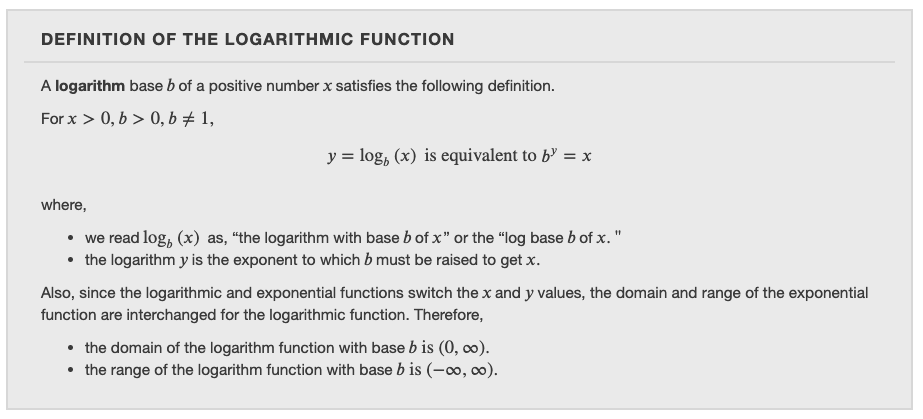
\includegraphics[width=\textwidth]{log_definition.png}

\end{definition*}


\begin{definition*}[Properties of Logarithms]\hfill
If $a > 0$, $b > 0$, $c > 0$, $b \neq 1$, and $r$ is any real number, then
\begin{itemize}
\item inverse property: $\log_b b^x = x$ and $b^{\log_b x} = x$
\item Special Cases
	\begin{enumerate} 
	\item $\log_b 1 = 0$
	\item $\log_b b = 1$
	\end{enumerate}
\item product property: $\log_b(ac) = \log_b(a) + \log_b(c)$ 
\item quotient property: $\log_b\left(\frac{a}{c}\right) = \log_b(a) - \log_b(c)$ 
\item power property: $\log_b(a^r) = r\log_b(a)$
\end{itemize}
\end{definition*}

\vfill
\noindent We want to show that $\log(A^n) = n\log(A)$ when $A >0$ and $n$ is any real number. Let $A = 10^x$, notice $A >0$. We compute
\begin{align*}
\log(A^n) &= \log(10^x)^n &\text{(substitute for $A$)}\\
&= \log(10^{nx}) &\text{(rewrite $(10^x)^n$)}\\
&= nx &\text{(inverse property of logs)}\\
&=n(\log A). &\text{(substitute for $x$)}
\end{align*}
Thus, $\log(A^n) = n\log(A)$.

%WRITE UP the proofs for the other two log properties.
%\prod_{i=1}^n n is the code for writing a product in product notation.


\end{document}